% Shared preamble for the Generative AI (CS 782/882, Fall 2026) lecture notes.
% Each weekNN-notes.tex file inlines this block so it compiles on its own.
\documentclass[11pt]{article}
\usepackage[margin=1in]{geometry}
\usepackage[T1]{fontenc}
\usepackage[utf8]{inputenc}
\usepackage{lmodern}
\usepackage{amsmath,amssymb,amsthm,mathtools,bm}
\usepackage{enumitem}
\usepackage{graphicx}
\usepackage{booktabs}
\usepackage{xcolor}
\usepackage{tikz}
\usetikzlibrary{arrows.meta,positioning,calc,shapes}
\usepackage{listings}
\usepackage[colorlinks=true,linkcolor=blue!60!black,urlcolor=blue!60!black,citecolor=blue!60!black]{hyperref}

\newcommand{\E}{\mathbb{E}}
\newcommand{\Var}{\mathrm{Var}}
\newcommand{\KL}{\mathrm{KL}}
\newcommand{\given}{\,\vert\,}
\newcommand{\R}{\mathbb{R}}
\DeclareMathOperator*{\argmax}{arg\,max}
\DeclareMathOperator*{\argmin}{arg\,min}
\newtheorem{theorem}{Theorem}
\newtheorem{lemma}{Lemma}
\newtheorem{definition}{Definition}
\theoremstyle{remark}
\newtheorem*{remark}{Remark}

\lstset{basicstyle=\ttfamily\small,breaklines=true,frame=single,columns=fullflexible}

% Week 7 additions (after the shared preamble)
\newcommand{\plain}[1]{\medskip\noindent\textit{Plain English:} #1\medskip}
\newcommand{\sg}{\operatorname{sg}}

\title{Week 7 Lecture Notes: World Models}
\author{Hong Qin, Old Dominion University}
\date{Fall 2026}

\begin{document}
\maketitle

\begin{center}
\textit{Audience:} graduate students who have completed the VAE (Week 2), autoregressive and LSTM (Week 4), diffusion (Week 5), and transformer (Week 6) material.\\
\textit{Goal:} understand what a world model is, how the V/M/C decomposition of Ha and Schmidhuber works, how an agent can be trained inside its own imagination, how the Dreamer line refined that idea, where the same idea appears in current research, and how to present a research paper well.
\end{center}

\tableofcontents
\bigskip
\hrule
\bigskip

% =====================================================================
\section{Topic 1: Predictive Modeling of Latent States or Environments}
% =====================================================================

\subsection*{Plain-English summary first}

A \textbf{world model} is a learned, compact, predictive model of an environment. Once an agent has one, it can plan ahead, train inside imagined rollouts instead of the real world, or simply use the model's representation for downstream tasks. The most influential modern formulation is Ha and Schmidhuber (2018), which factors the world model into three pieces you have already met in this course:

\begin{itemize}[leftmargin=1.4em]
  \item a \textbf{Vision} module (V) that encodes a raw observation into a small latent vector (a VAE, Week 2);
  \item a \textbf{Memory} module (M) that predicts the next latent given the current latent and the action (a mixture-density LSTM, combining the LSTM of Week 4 with a mixture-density output head);
  \item a tiny \textbf{Controller} (C) that maps the latent state and the memory state to an action.
\end{itemize}

This section introduces the framework and explains why splitting an agent into these three parts is a useful decomposition.

\subsection{The agent-environment setup}

We borrow the framing of reinforcement learning (RL). At each timestep $t$, the agent receives an observation $o_t$ from the environment, picks an action $a_t$, and receives a reward $r_t$ together with a new observation $o_{t+1}$. The goal is to maximize the expected discounted return
\begin{equation}
  J \;=\; \E\!\left[\sum_{t=0}^{\infty} \gamma^{t} r_t\right], \qquad \gamma \in (0,1).
  \label{eq:return}
\end{equation}

\plain{The discount $\gamma$ says that a reward received now is worth more than the same reward received later; with $\gamma$ close to 1 the agent is patient, with $\gamma$ close to 0 it is greedy. Equation~\eqref{eq:return} is the single number every RL method is trying to make large.}

Two broad ways to make $J$ large:

\begin{itemize}[leftmargin=1.4em]
  \item \textbf{Model-free RL.} Learn the policy $\pi(a_t \given o_t)$ (or a value function) directly from interaction. Examples: REINFORCE, DQN, PPO. Simple and robust, but sample-inefficient: you need a lot of real environment steps.
  \item \textbf{Model-based RL.} Learn a model of the environment (its dynamics and its reward), then use the model to plan or to train a policy. Sample-efficient (one real step can be replayed into many imagined steps), but only as good as the model.
\end{itemize}

World models are the centerpiece of modern model-based RL.

\subsection{The V/M/C architecture of Ha and Schmidhuber (2018)}

\begin{center}
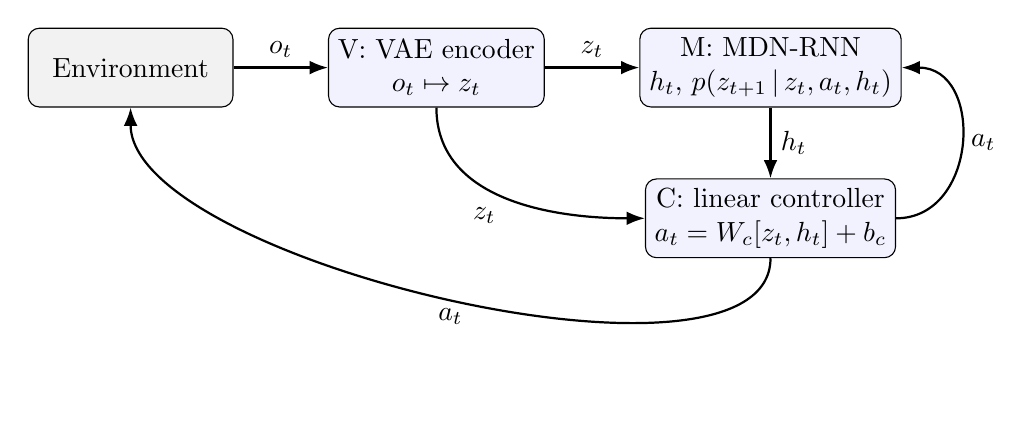
\begin{tikzpicture}[
  node distance=9mm and 12mm,
  box/.style={draw, rounded corners, minimum width=2.6cm, minimum height=1.0cm, align=center, fill=blue!5},
  env/.style={draw, rounded corners, minimum width=2.6cm, minimum height=1.0cm, align=center, fill=gray!10},
  arr/.style={-Latex, thick}
]
  \node[env] (env) {Environment};
  \node[box, right=of env] (V) {V: VAE encoder\\ $o_t \mapsto z_t$};
  \node[box, right=of V] (M) {M: MDN-RNN\\ $h_t$, $p(z_{t+1}\given z_t,a_t,h_t)$};
  \node[box, below=of M] (C) {C: linear controller\\ $a_t = W_c[z_t,h_t]+b_c$};

  \draw[arr] (env) to node[above] {$o_t$} (V);
  \draw[arr] (V) to node[above] {$z_t$} (M);
  \draw[arr] (V.south) to[out=-90,in=180] node[below left] {$z_t$} (C.west);
  \draw[arr] (M) to node[right] {$h_t$} (C);
  \draw[arr] (C.south) to[out=-90,in=-90,looseness=0.6] node[below] {$a_t$} (env.south);
  \draw[arr] (C.east) to[out=0,in=0,looseness=1.4] node[right] {$a_t$} (M.east);
\end{tikzpicture}
\end{center}

\noindent\textit{The V/M/C loop. The observation is compressed by V, the memory M carries the history and predicts the future, and the small controller C picks the action from $[z_t, h_t]$. The action is fed back to both the environment and the memory.}

\subsubsection*{V: the vision module}

V is a variational autoencoder trained on a buffer of observations (in the paper, $64\times 64\times 3$ frames from the CarRacing environment collected under a random policy). The encoder produces a Gaussian over a latent of dimension about $32$:
\begin{equation}
  q_\phi(z_t \given o_t) \;=\; \mathcal N\!\big(\mu_\phi(o_t),\, \mathrm{diag}\,\sigma^2_\phi(o_t)\big),
  \qquad
  z_t \;=\; \mu_\phi(o_t) + \sigma_\phi(o_t)\odot \varepsilon,\ \ \varepsilon\sim\mathcal N(0,I).
  \label{eq:venc}
\end{equation}
The VAE is trained with the usual ELBO (reconstruction minus a KL to the standard normal prior), then the encoder and decoder are \emph{frozen}.

\plain{V does exactly what the Week 2 VAE did on Fashion-MNIST, except that its inputs are game frames. Its only job is to turn a picture into a short vector $z_t$ that keeps what matters (road shape, car position) and throws away what does not (pixel-level texture). Because V is frozen after training, everything downstream can rely on a stable code.}

\subsubsection*{M: the memory module (MDN-RNN)}

M is an LSTM whose output head is a mixture density network. Given the current latent $z_t$, the action $a_t$, and the recurrent state $h_t$, it predicts a distribution over the next latent:
\begin{equation}
  p\!\left(z_{t+1} \given z_t,\, a_t,\, h_t\right) \;=\; \mathrm{MDN}\!\left(\mathrm{RNN}(z_t, a_t, h_t)\right).
  \label{eq:mdnrnn}
\end{equation}
Spelled out, the RNN updates its hidden state and the MDN head reads off the parameters of a Gaussian mixture with $K$ components:
\begin{align}
  h_{t+1} &= \mathrm{LSTM}\big([z_t, a_t],\, h_t\big), \label{eq:rnn}\\
  (\pi_{k}, \mu_{k}, \sigma_{k})_{k=1}^{K} &= \mathrm{MLP}(h_{t+1}), \qquad \pi_k \ge 0,\ \ \sum_{k=1}^K \pi_k = 1, \label{eq:mdnhead}\\
  p(z_{t+1}\given z_t, a_t, h_t) &= \sum_{k=1}^{K} \pi_k\, \mathcal N\!\big(z_{t+1};\, \mu_k,\, \sigma_k^2 I\big). \label{eq:mixture}
\end{align}
M is trained by maximizing the log-likelihood of the next latents on recorded rollouts, that is, by minimizing
\begin{equation}
  \mathcal L_M \;=\; -\sum_{t} \log \sum_{k=1}^{K} \pi_k\, \mathcal N\!\big(z_{t+1};\, \mu_k, \sigma_k^2 I\big).
  \label{eq:mdnloss}
\end{equation}
The original paper also introduces a temperature $\tau$ that scales the mixture variances when sampling, which lets you make the imagined world more or less unpredictable than the data.

\plain{The LSTM is the Week 4 sequence model; its hidden state $h_t$ is a running summary of everything the agent has seen so far. The mixture head is the important new piece. A single Gaussian can only say ``the next state is around here.'' A mixture can say ``with probability 0.6 the road bends left, with probability 0.4 it bends right,'' which is what a branching environment requires. Predicting the mean of two branches would put the car in the wall between them.}

\subsubsection*{C: the controller}

C is a tiny linear policy from the concatenated latent and memory state to the action:
\begin{equation}
  a_t \;=\; W_c\,[z_t,\, h_t] + b_c .
  \label{eq:controller}
\end{equation}
For CarRacing this is roughly $1000$ parameters in total. It is trained with the \textbf{CMA-ES} evolutionary algorithm rather than backpropagation: a population of parameter vectors is sampled, each is evaluated by running episodes, and the sampling distribution is moved toward the better-scoring members.

\plain{Because C is so small, black-box search is fast enough. This sidesteps the hard problem of backpropagating reward through a long chain of stochastic RNN steps. The reward signal touches only C; V and M never see a reward.}

\subsection{Why factor the agent this way?}

\begin{itemize}[leftmargin=1.4em]
  \item \textbf{Reusability.} V and M are generative and reward-free. A vision module trained on a domain can serve many controllers for many tasks in that domain without retraining.
  \item \textbf{Sample efficiency.} Generative training needs no reward labels and can use any collected experience, including random-policy rollouts.
  \item \textbf{Evolvability.} C is small enough to evolve; CMA-ES treats it as a black box.
  \item \textbf{Interpretability.} You can inspect the decoder reconstructions to debug V, and sample MDN-RNN rollouts to debug M, independently of how well the agent plays.
\end{itemize}

\subsection*{Plain-English payoff}

The big networks do the unsupervised work: V learns to see, M learns to predict. The reward, which is the scarce and noisy signal, is spent only on a thousand-parameter controller. That separation is why the agent learns CarRacing from surprisingly few real interactions, and it is the same separation (representation first, task-specific head last) that reappears in foundation models. Topic 2 turns M into a simulator and trains the agent inside it.

% =====================================================================
\section{Topic 2: Planning, Imagination, and Structured Reasoning}
% =====================================================================

\subsection*{Plain-English summary first}

Once you have a fast predictive model of the environment, you can train the agent \emph{inside} the model: roll out imagined trajectories instead of spending expensive real interactions. This ``dreaming'' is the central use of world models in RL, and it is why model-based RL can be far more sample-efficient than model-free RL when the model is good enough. This section walks through in-dream training in the Ha and Schmidhuber setup, explains why it can fail, and then summarizes the Dreamer line of work (PlaNet, Dreamer, DreamerV2, DreamerV3) that became the modern benchmark for model-based RL.

\subsection{In-dream training}

In Ha and Schmidhuber (2018), the controller can be trained entirely inside the world model:

\begin{enumerate}[leftmargin=1.6em]
  \item \textbf{Initialize.} Encode a starting observation $o_0$ with V to get $z_0$; set the RNN state $h_0$.
  \item \textbf{Roll out in imagination.} For $t = 0, 1, \dots, H-1$:
  \begin{equation}
    a_t = W_c[z_t, h_t] + b_c, \qquad
    z_{t+1} \sim p(z_{t+1} \given z_t, a_t, h_t), \qquad
    h_{t+1} = \mathrm{LSTM}([z_t, a_t], h_t).
    \label{eq:imagine}
  \end{equation}
  \item \textbf{Score the dream.} Use a reward $\hat r_t$ predicted alongside the latent (the original paper used a separate small reward or ``done'' head).
  \item \textbf{Improve the controller.} Choose $\theta_C = (W_c, b_c)$ to maximize the imagined return
  \begin{equation}
    \hat J(\theta_C) \;=\; \E_{\text{model}}\!\left[\sum_{t=0}^{H-1} \gamma^t\, \hat r_t\right]
    \label{eq:imagined-return}
  \end{equation}
  with CMA-ES.
\end{enumerate}

The agent never touches a real environment step during this phase. Real interaction is used only to collect data for V and M.

\plain{Equation~\eqref{eq:imagine} is the same loop as the real environment, except that the ``environment'' box in the diagram is replaced by M. Since M runs on a GPU and never has to render pixels, thousands of imagined episodes cost about what a handful of real ones would. Equation~\eqref{eq:imagined-return} is the real objective~\eqref{eq:return} with the true rewards replaced by the model's guesses.}

\subsection{Why this works, and when it does not}

The policy is only as good as the world model is accurate. Two failure modes:

\begin{itemize}[leftmargin=1.4em]
  \item \textbf{Model exploitation.} The controller finds states the model predicts incorrectly (typically far from the training distribution) and learns a policy that scores high imagined reward by visiting them. Real-environment performance is then terrible.
  \item \textbf{Compounding error.} Long rollouts accumulate a prediction error at every step. If the one-step error is $\epsilon$, an $H$-step rollout can drift on the order of $H\epsilon$ or worse, because each error feeds the next input. Short rollouts work better; long rollouts drift off the data manifold.
\end{itemize}

Mitigations that appear in the literature: ensembles of world models (Janner et al., 2019), short imagined rollouts mixed with real experience (the original Ha paper does this), and conservative policy-improvement objectives that bound the gap between imagined and real performance. Raising the sampling temperature $\tau$ in M is another cheap trick: a noisier dream is harder to exploit.

\plain{Think of the model as a flight simulator. If the simulator has a bug that lets the plane fly through mountains, a pilot trained only in the simulator will learn to fly through mountains. The remedies are to fix the simulator (better data, ensembles), to keep sessions short, and to make the simulator slightly harsher than reality.}

\subsection{The Dreamer line of work}

Hafner and colleagues extended the framework into a sequence of increasingly capable systems built on the same decomposition (a latent state, a learned dynamics, and a policy) with much better engineering.

\subsubsection*{PlaNet (Hafner et al., 2018): latent planning with an RSSM}

PlaNet introduced the \textbf{recurrent state-space model} (RSSM), which keeps both a deterministic and a stochastic latent:
\begin{align}
  \text{deterministic:} \quad & h_t = f_\theta(h_{t-1}, z_{t-1}, a_{t-1}), \label{eq:rssm-det}\\
  \text{prior (transition):} \quad & z_t \sim p_\theta(z_t \given h_t), \label{eq:rssm-prior}\\
  \text{posterior (representation):} \quad & z_t \sim q_\phi(z_t \given h_t, o_t), \label{eq:rssm-post}\\
  \text{decoders:} \quad & o_t \sim p_\theta(o_t \given h_t, z_t), \qquad r_t \sim p_\theta(r_t \given h_t, z_t). \label{eq:rssm-dec}
\end{align}
The world model is trained with an ELBO-style objective, summed over time:
\begin{equation}
  \mathcal L_{\text{WM}} \;=\; \sum_t \Big(
    -\,\E_{q}\big[\log p_\theta(o_t\given h_t,z_t)\big]
    \;-\;\E_{q}\big[\log p_\theta(r_t\given h_t,z_t)\big]
    \;+\;\beta\,\KL\!\big(q_\phi(z_t\given h_t,o_t)\,\|\,p_\theta(z_t\given h_t)\big)
  \Big).
  \label{eq:rssm-loss}
\end{equation}
PlaNet has no learned controller: at each real timestep it plans in latent space with the cross-entropy method (sample action sequences, roll them through the RSSM, keep the best, refit, repeat).

\plain{Compare with V/M: the posterior $q_\phi(z_t\given h_t,o_t)$ plays the role of V, the prior $p_\theta(z_t\given h_t)$ plays the role of M's one-step prediction, and the deterministic $h_t$ is the LSTM memory. The KL term is the new ingredient: it pushes the prediction made \emph{without} seeing $o_t$ to agree with the encoding made \emph{with} $o_t$, which is exactly what makes the model usable for dreaming, where $o_t$ is unavailable.}

\subsubsection*{Dreamer / DreamerV1 (Hafner et al., 2020): actor-critic in latent space}

Dreamer replaced online planning with a learned actor and critic trained purely inside the world model. Starting from posterior states drawn from replayed real data, it imagines $H$ steps with the prior:
\begin{equation}
  a_\tau \sim \pi_\psi(a_\tau \given s_\tau), \qquad
  s_{\tau+1} \sim p_\theta(s_{\tau+1}\given s_\tau, a_\tau), \qquad
  \hat r_\tau = \E\big[p_\theta(r_\tau \given s_\tau)\big], \qquad s_\tau = (h_\tau, z_\tau).
  \label{eq:dreamer-imagine}
\end{equation}
The critic $v_\xi(s)$ is regressed onto a $\lambda$-return computed along the imagined trajectory,
\begin{equation}
  V^\lambda_\tau \;=\; \hat r_\tau + \gamma\Big[(1-\lambda)\, v_\xi(s_{\tau+1}) + \lambda\, V^\lambda_{\tau+1}\Big],
  \qquad V^\lambda_{H} = v_\xi(s_H),
  \label{eq:lambda-return}
\end{equation}
and the actor and critic are trained with
\begin{equation}
  \mathcal L_{\text{actor}}(\psi) = -\sum_{\tau=t}^{t+H-1} V^\lambda_\tau, \qquad
  \mathcal L_{\text{critic}}(\xi) = \sum_{\tau=t}^{t+H-1} \tfrac12\big(v_\xi(s_\tau) - \sg(V^\lambda_\tau)\big)^2,
  \label{eq:dreamer-ac}
\end{equation}
where $\sg(\cdot)$ stops the gradient. The key technical move is that the actor loss is differentiated \emph{through the dynamics model}: because the latent transition is continuous and reparameterized, gradients flow from the imagined return back through $s_{\tau+1}, a_\tau, s_\tau, \dots$ into $\psi$.

\plain{The critic is a learned estimate of ``how much reward will I collect from this latent state onward.'' The $\lambda$-return in~\eqref{eq:lambda-return} mixes actual imagined rewards over a few steps with the critic's estimate of the rest, so the actor is not limited to what happens inside the $H$-step horizon. The actor is then improved by plain gradient ascent on that estimate, which is possible only because the whole imagined trajectory is differentiable. This is exactly what CMA-ES in the Ha and Schmidhuber setup was avoiding; Dreamer's smooth, low-variance latent dynamics make it viable.}

\subsubsection*{DreamerV2 (Hafner et al., 2021): discrete latents and KL balancing}

DreamerV2 replaced the Gaussian stochastic latent with a vector of categorical variables (a grid of one-hot codes, trained with straight-through gradients) and split the KL term so that the prior and posterior are pulled toward each other at different rates:
\begin{equation}
  \mathcal L_{\KL} \;=\; \alpha\,\KL\!\big(\sg(q)\,\|\,p\big) + (1-\alpha)\,\KL\!\big(q\,\|\,\sg(p)\big), \qquad \alpha \approx 0.8 .
  \label{eq:klbalance}
\end{equation}
It was the first model-based agent to beat the strongest model-free baselines on Atari.

\plain{Discrete latents give the model a vocabulary of ``situations'' instead of a smooth cloud, which turned out to be a better fit for game-like environments. KL balancing says: mostly train the predictor to match the encoder (weight $\alpha$), and only gently train the encoder to be predictable (weight $1-\alpha$). Without it, the encoder can collapse toward the prior and stop carrying information.}

\subsubsection*{DreamerV3 (Hafner et al., 2023): one configuration for over 150 tasks}

DreamerV3 is the current reference for general-purpose model-based RL. With a single fixed set of hyperparameters it works across Atari, continuous control, Minecraft, and robotic manipulation, and it was the first system to collect diamonds in Minecraft from scratch without curricula or human data. The engineering ingredients (symlog reward transforms, free-bits on the KL, percentile-normalized returns) are all about making the same objective robust to wildly different reward scales.

\subsection{Connection to LLM-based agents and to JEPA}

A large language model can be viewed as an \emph{implicit} world model over the space of text. When you prompt an LLM to think step by step, you are rolling out an imagined trajectory in its world model and using it to plan. The agent frameworks from Week 6 do the same thing to plan multi-step tool use.

LeCun's JEPA proposal (2022) is an explicit attempt to build dedicated world models for non-language data with self-supervised learning. Its prediction objective lives in \emph{representation} space rather than pixel space: encode a context $x$ and a target $y$, then train a predictor to map the context embedding (plus a latent $u$ that absorbs what the context cannot determine) onto the target embedding,
\begin{equation}
  \min_{\theta}\ \E\Big[\, D\big(\, \mathrm{Pred}_\theta(s_x, u),\ \sg(s_y)\,\big) \Big],
  \qquad s_x = \mathrm{Enc}(x),\ \ s_y = \mathrm{Enc}(y),
  \label{eq:jepa}
\end{equation}
with a regularizer that keeps the embeddings from collapsing to a constant.

\plain{A pixel-space predictor must reproduce every leaf on every tree. JEPA argues that a world model should predict only what is predictable and abstract, so it compares predictions with targets in the learned embedding space. This is the same instinct as V in Topic 1 (predict in latent space, not pixel space), pushed one step further by dropping the decoder entirely.}

\subsection*{Plain-English payoff}

Whether the world model is explicit (Dreamer) or implicit (an LLM), the idea that competent behavior requires an internal predictive model of the world is now mainstream. The practical lessons transfer: keep prediction in a compact latent space, keep imagined rollouts short, and always evaluate in the real environment because a policy can score well in a broken dream.

% =====================================================================
\section{Topic 3: Linking World Models to Current Research Directions}
% =====================================================================

\subsection*{Plain-English summary first}

World models have had a renaissance since 2023. The ideas from Topics 1 and 2 (predict the future, plan inside the predictor, train a policy from imagined rollouts) now show up in places that do not call themselves world models: foundation video generators, robot foundation models, and the implicit world modeling that large language models do when they reason. This section is a tour so that you can recognize the framework in modern papers and place your project against the current landscape.

\subsection{Video generation as world modeling}

Text-to-video systems (Sora from OpenAI, Veo from Google, Movie Gen from Meta) are trained on very large video datasets to model future frames conditioned on a text prompt. Abstractly, they learn
\begin{equation}
  p_\theta\big(x_{1:T} \given c\big) \quad\text{or, autoregressively in time,}\quad p_\theta\big(x_{t+1} \given x_{1:t},\, c\big),
  \label{eq:video}
\end{equation}
where $x_t$ is a frame (in practice a compressed latent of a frame, as in Week 5's latent diffusion) and $c$ is the text condition. The result implicitly learns physics, object permanence, and basic causal structure. OpenAI framed Sora as a step toward ``general-purpose simulators of the physical world,'' which is the world-model framing.

Whether these are ``real'' world models is contested. They predict pixel evolution beautifully but have no explicit notion of objects, no inverse model for actions, and no planning loop. The pragmatic answer: they are world models for the narrow task of predicting plausible future frames, but not yet general-purpose world models suitable for arbitrary agent control.

\plain{Compare~\eqref{eq:video} with M's one-step predictor~\eqref{eq:mdnrnn}. The video model is the same object with three differences: the condition is text rather than an action, the state is a whole frame latent rather than a 32-dimensional code, and the sampler is a diffusion model rather than a Gaussian mixture. What is missing is the $a_t$: nothing lets an agent steer the rollout.}

\subsection{Genie: the playable world model}

Google DeepMind's Genie (2024) and Genie~2 (2024), trained on Internet video, generate playable 2D and (in Genie~2) interactive 3D environments from a single image prompt. The missing $a_t$ is put back: the generative model predicts the next frame conditioned on a discrete action,
\begin{equation}
  p_\theta\big(x_{t+1} \given x_{1:t},\, a_t\big), \qquad a_t \in \{1, \dots, A\},
  \label{eq:genie}
\end{equation}
where the action vocabulary is itself learned without action labels from the video (a latent action model infers which of $A$ discrete ``moves'' best explains the change between consecutive frames). This is the most direct realization of a Ha-and-Schmidhuber-style world model at Internet scale: you can drive it interactively.

\plain{Genie is M with a keyboard attached. Because nobody labels Internet video with joystick inputs, the model has to invent its own small set of actions by asking ``what few controls would explain how this frame turned into the next one?'' Once it has them, a user can press those controls and watch the dream respond.}

\subsection{Robot foundation models}

Large robot policy models (RT-1 in 2022, RT-2 in 2023, and the cross-embodiment RT-X dataset in 2023) are trained on very large collections of robot trajectories across many embodiments. They are not labeled world models in the V/M/C sense, but the structure is closely related: a perception network maps observations to a representation, and an autoregressive transformer predicts action sequences conditioned on a goal,
\begin{equation}
  \pi_\theta\big(a_{t:t+k} \given o_t,\, g\big), \qquad g = \text{language goal}.
  \label{eq:vla}
\end{equation}
The dynamics model is implicit (the physical robot embodies it) and the policy is integrated, but the family resemblance to Ha and Schmidhuber is clear. Follow-on work (Octo, OpenVLA, the $\pi_0$ family) makes the world-modeling component more explicit and lets one base model drive many platforms.

\plain{Here V is a vision-language backbone and C is a transformer head; M is the real world. The lesson from world models that carries over is the reuse of a large reward-free representation across many tasks and bodies.}

\subsection{World models inside LLM reasoning}

Interpretability work (Li et al., OthelloGPT, and many others since) has found that sequence models trained only to predict the next token learn internal representations that function like world models: they track entities, infer hidden state, and roll simulations forward. In OthelloGPT, a transformer trained on move sequences was shown, by linear probes, to represent the state of the board, even though it never saw a board. This is one mechanistic explanation for why chain-of-thought prompting helps: the model uses its implicit world model to imagine consequences before committing to an answer.

This is the bridge between Week 4 (autoregressive modeling), Week 6 (transformers), and this week. Modern large generative models are increasingly understood as containing implicit world models, and the practical advances in agent frameworks build on that.

\subsection{Where world models may matter for your project}

Even if your project is not about RL, the framework gives you vocabulary for:
\begin{itemize}[leftmargin=1.4em]
  \item any project where a generative model is used to \emph{simulate} something (synthetic data, what-if analysis, scenario planning) rather than only to sample from data;
  \item any project where an agent or pipeline takes multiple dependent steps (a tool-use agent, a multi-step analysis pipeline, a robot action sequence);
  \item any project on video, time-series, or sequence data where future prediction is part of the task.
\end{itemize}
If none of these apply, the material is still part of the modern AI vocabulary and will appear in papers you read after the course.

\subsection*{Plain-English payoff}

The recurring pattern across video generators, Genie, robot policies, and LLMs is: a learned encoder into a compact state, a learned predictor of what comes next (conditioned on text, action, or goal), and, when there is an agent, a small policy on top. When you meet a new system, ask three questions: what is the state, what is being predicted, and is there an action? The answers tell you which parts of the V/M/C picture the system has and which it lacks.

% =====================================================================
\section{Topic 4: Technical Communication Through Paper Presentation}
% =====================================================================

\subsection*{Plain-English summary first}

Presenting a paper well is a separate skill from understanding it. This section is the practical how-to for a recorded 12-to-15-minute research paper presentation: a structure that works, slide-design principles, how to pitch technical depth to a mixed audience, recording tools, common failure modes, and accessibility expectations. Most of the advice applies to any scientific talk; the specifics are tuned for an asynchronous recorded format.

\subsection{A six-section structure that works}

Adjust the lengths to your paper's emphasis, but keep all six sections.

\begin{enumerate}[leftmargin=1.6em]
  \item \textbf{Title slide and the ``why care'' opener (1 minute).} Paper title, authors, venue, year. One sentence on why the paper interests you, in language a classmate outside your sub-area can follow.
  \item \textbf{Problem and prior work (2 to 3 minutes).} What problem is solved? What was the state of the art, and what was wrong with it? Two or three citations suffice.
  \item \textbf{The method (4 to 5 minutes).} The longest section. Show diagrams and equations. One diagram per slide; for a key equation, explain every symbol.
  \item \textbf{Results (2 to 3 minutes).} Two or three figures, not all of them. Be specific about what was compared, what the baseline was, and what improved.
  \item \textbf{Limitations and open questions (1 to 2 minutes).} The most-skipped and most valuable section. What does the paper not do? What would have to change for it to scale? What follow-up work exists?
  \item \textbf{Relevance to the course or your project (1 minute).} Close the loop with the model families studied in this course or with your own project.
\end{enumerate}

\subsection{Slide design and speaking calibration}

\begin{itemize}[leftmargin=1.4em]
  \item One idea per slide; body text at least 24\,pt, titles 32\,pt (video compression erases small text).
  \item Diagrams over words; equations are fine if you walk through them aloud.
  \item Cite as you go (author, year at the bottom of the slide); reuse the paper's own figures and credit them.
  \item Assume the standard methods (VAE, GAN, transformer, diffusion); do not assume sub-field notation. Aim for ``an interested classmate could follow without pausing.'' If you catch yourself saying ``by routine manipulation,'' slow down there.
  \item Pace: about 150 words per minute, so 12 to 15 minutes is roughly 1800 to 2250 words of script. Speak from notes rather than reading verbatim.
\end{itemize}

\subsection{Recording tools, failure modes, and accessibility}

Any familiar tool is acceptable: ODU Panopto, Zoom or Teams local recording, Loom, OBS Studio, QuickTime, or Xbox Game Bar. Captions or an equivalent transcript are required; either use a tool with auto-captions and correct the major errors, or submit a script as a separate PDF or text file.

\medskip
\noindent\textbf{Pre-submission checklist}
\begin{itemize}[leftmargin=1.4em, itemsep=1pt]
  \item[$\square$] All six sections present, in order, within the 12-to-15-minute window (hard ceiling 15 minutes; rehearsed with a timer).
  \item[$\square$] No slide is read verbatim; the voice adds information the slide does not.
  \item[$\square$] Planned 2-to-3-second pauses after each main point so viewers can read figures and equations.
  \item[$\square$] Audio tested first: no hum, no background noise, adequate volume.
  \item[$\square$] Limitations section is substantive, not a formality.
  \item[$\square$] Every reused figure and every non-original claim is cited on the slide.
  \item[$\square$] Captions reviewed, or a transcript file included with the submission.
\end{itemize}

\subsection*{Plain-English payoff}

A talk that only presents the wins reads as marketing; the limitations section is where you demonstrate critical thinking. Rehearse with a timer, test the audio, and end by telling the audience why the paper matters to what they already know.

% =====================================================================
\section*{References}
\addcontentsline{toc}{section}{References}
% =====================================================================

\begin{enumerate}[leftmargin=2em, label={[\arabic*]}, itemsep=2pt]
  \item D. Foster, \emph{Generative Deep Learning}, 2nd ed., O'Reilly, 2023. Chapter 12, ``World Models.''
  \item D. Ha and J. Schmidhuber, ``World Models,'' NeurIPS 2018. \href{https://arxiv.org/abs/1803.10122}{arXiv:1803.10122}. Interactive companion: \url{https://worldmodels.github.io/}.
  \item J. Schmidhuber, ``On Learning to Think: Algorithmic Information Theory for Novel Combinations of Reinforcement Learning Controllers and Recurrent Neural World Models,'' 2015. \href{https://arxiv.org/abs/1511.09249}{arXiv:1511.09249}.
  \item D. Hafner et al., ``Learning Latent Dynamics for Planning from Pixels'' (PlaNet), ICML 2019. \href{https://arxiv.org/abs/1811.04551}{arXiv:1811.04551}.
  \item D. Hafner et al., ``Dream to Control: Learning Behaviors by Latent Imagination'' (DreamerV1), ICLR 2020. \href{https://arxiv.org/abs/1912.01603}{arXiv:1912.01603}.
  \item D. Hafner et al., ``Mastering Atari with Discrete World Models'' (DreamerV2), ICLR 2021. \href{https://arxiv.org/abs/2010.02193}{arXiv:2010.02193}.
  \item D. Hafner et al., ``Mastering Diverse Domains through World Models'' (DreamerV3), 2023. \href{https://arxiv.org/abs/2301.04104}{arXiv:2301.04104}.
  \item M. Janner et al., ``When to Trust Your Model: Model-Based Policy Optimization,'' NeurIPS 2019. \href{https://arxiv.org/abs/1906.08253}{arXiv:1906.08253}.
  \item Y. LeCun, ``A Path Towards Autonomous Machine Intelligence'' (JEPA), OpenReview, 2022. \url{https://openreview.net/pdf?id=BZ5a1r-kVsf}.
  \item OpenAI, ``Video generation models as world simulators'' (Sora technical report), 2024. \url{https://openai.com/research/video-generation-models-as-world-simulators}.
  \item J. Bruce et al., ``Genie: Generative Interactive Environments,'' ICML 2024. \href{https://arxiv.org/abs/2402.15391}{arXiv:2402.15391}. Genie 2 announcement: Google DeepMind blog, 2024.
  \item Open X-Embodiment Collaboration, ``Open X-Embodiment: Robotic Learning Datasets and RT-X Models,'' 2023. \href{https://arxiv.org/abs/2310.08864}{arXiv:2310.08864}.
  \item A. Brohan et al., ``RT-2: Vision-Language-Action Models Transfer Web Knowledge to Robotic Control,'' CoRL 2023. \href{https://arxiv.org/abs/2307.15818}{arXiv:2307.15818}.
  \item K. Li et al., ``Emergent World Representations: Exploring a Sequence Model Trained on a Synthetic Task'' (OthelloGPT), ICLR 2023. \href{https://arxiv.org/abs/2210.13382}{arXiv:2210.13382}.
  \item S. Keshav, ``How to Read a Paper,'' ACM SIGCOMM Computer Communication Review, 2007.
  \item S. Peyton Jones, ``How to give a great research talk,'' Microsoft Research. \url{https://www.microsoft.com/en-us/research/academic-program/give-great-research-talk/}.
\end{enumerate}

\end{document}
